\clearpage

\section{Evaluation}
\label{cp6:evaluation}


The goal of our evaluation is to investigate whether text automatically identified
as relevant to a task and shown to a developer assist them to complete their software task.
This evaluation helps answer: 


\medskip
\begin{bluequote}
    \textit{ Does text automatically identified by semantic-based techniques help a 
    developer more effectively complete a software development task?} 
\end{bluequote}


To answer this question, we detail a controlled experiment where participants 
had to complete \red{two} programming tasks when assisted (or not) by a
 tool that embeds such a semantic-based technique (\red{Section~\ref{}}). 


We report metrics related to the text that participants in the experiment indicated as helpful to the task-at-hand, their agreement on the extent to which the text automatically identified by our tool 
assisted them, and how complete were their solutions, as measured by test cases that judged
their code.


\subsection{Experimental Design}

\clearpage

\begin{figure}
    \centering
    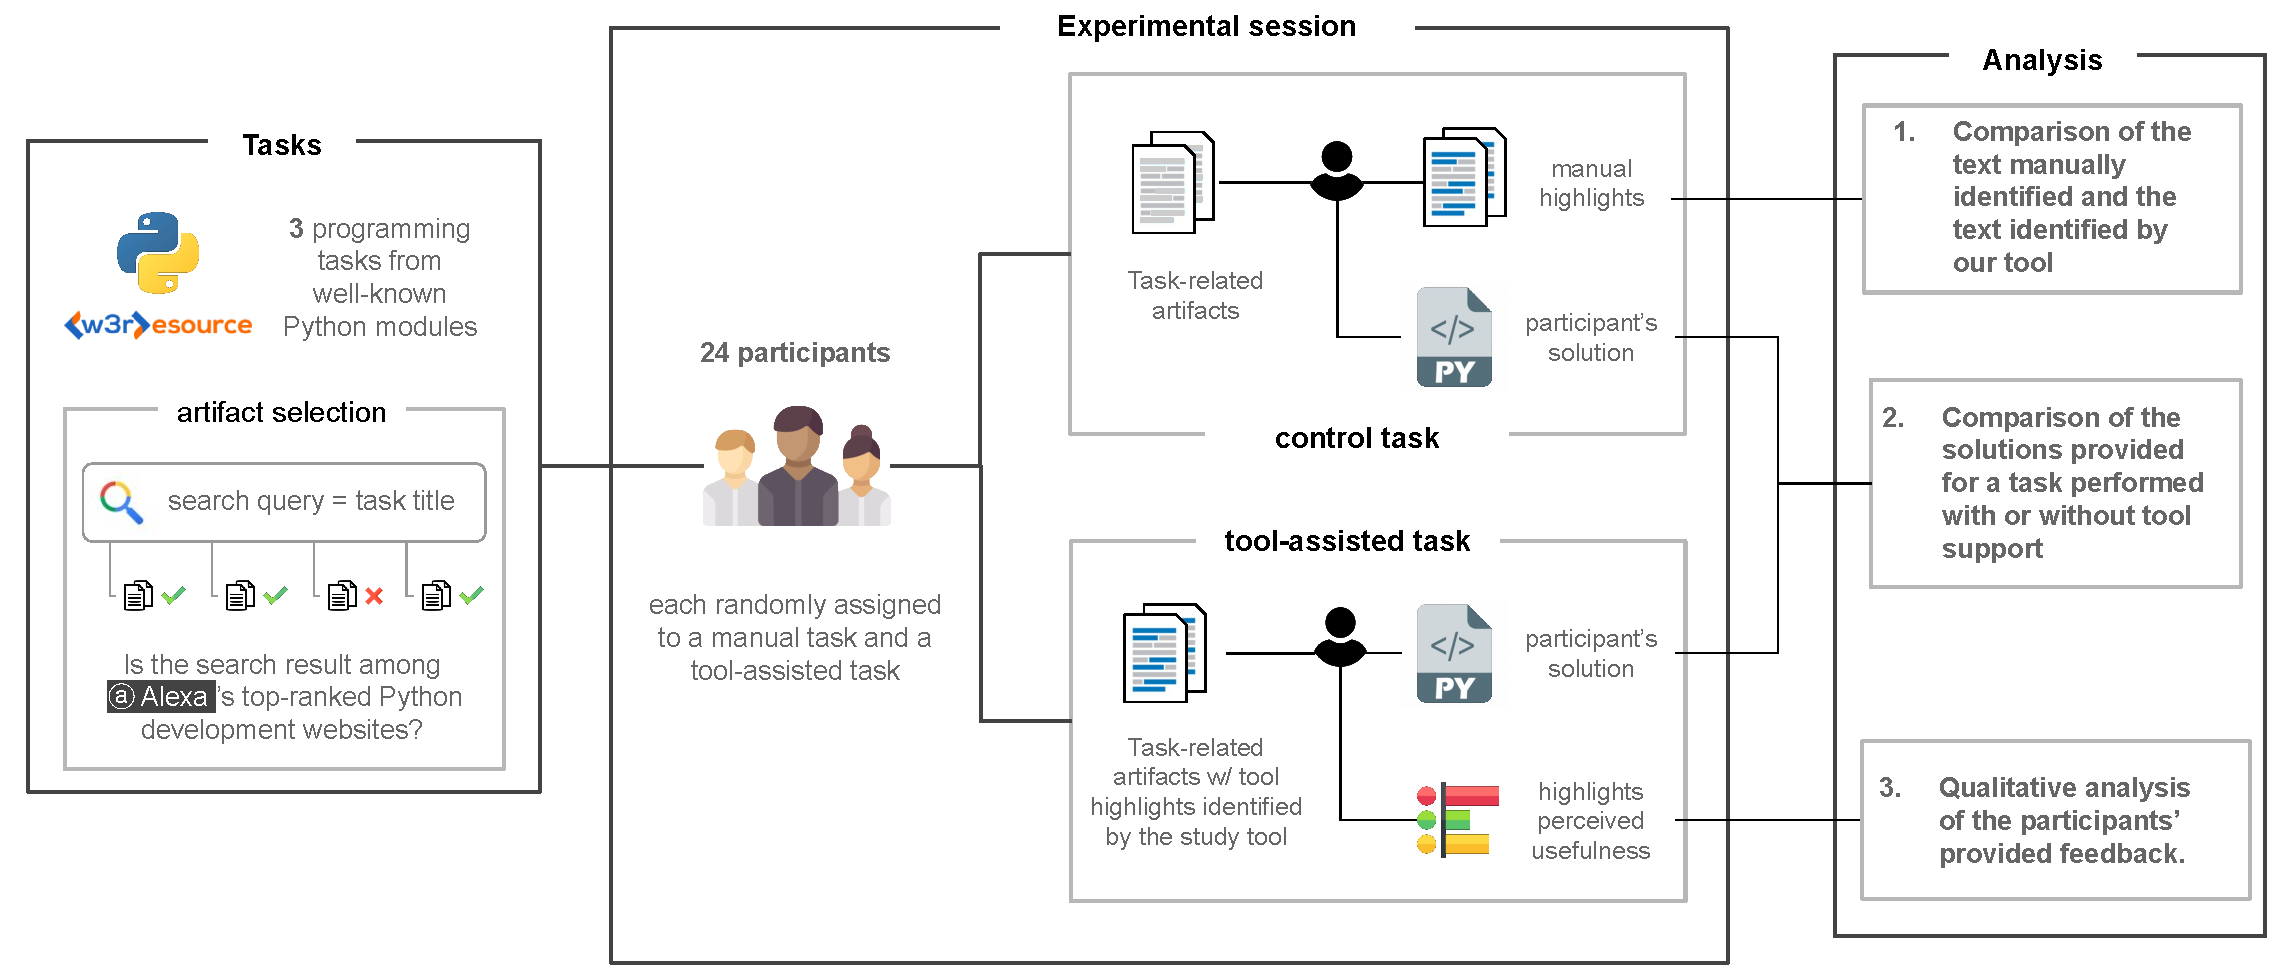
\includegraphics[width=1.\textwidth]{cp6/tool-experiment-pipeline}
    \caption{Overview of the study design and outcomes}
    \label{fig:cp6-experiment-overview}
\end{figure}

\clearpage

\subsubsection{Participants}



We advertised our study to third and fourth-year Computer Science students at the University of British Columbia. 
At this point in the curriculum, students should be familiar with \red{Python} and they should be able to come up with a solution 
for a software task when provided with artifacts containing information for that task.


Students were offered the opportunity to enter a raffle for one of two \red{\$50} online shopping gift cards.
We obtained answers from a total of \red{\#} students. \red{Demographics}


\subsubsection{Tasks}

Due to our target population, we scope tasks in our experiment to  
feature requests obtained from popular Python GitHub repos,
which encompass a social network crawler (\textit{Sherlock}),
a web-archiving tool (\textit{ArchiveBox}), and a \red{last project}.



We manually inspected each of the feature requests available in these repos, identifying
feature requests that
\textit{(1)}  required understanding interactions between different and well-known Python modules, 
\textit{(2)}  had pull requests merged to the repo's main branch and that
\textit{(3)}  had medium or small size changes in no more than two files (\red{$\le 300$ LOC}).


These criteria are based on the fact that we need tasks that are easy to understand and that are self-contained enough so that a student can come up with a solution to them in the amount of time allotted in our experimental procedures (Section~\ref{cp6:evaluation-procedures}).
According to these requirements, we selected the following feature requests:


\begin{itemize}
    \item \texttt{BeautifulSoup}: use BeautifulSoup4 to parse Google chrome bookmark dumps\footnote{https://github.com/ArchiveBox/ArchiveBox/pull/20}
    \item  \texttt{Threads}: use multiprocessing and subprocess modules to find all the files that contain some value\footnote{https://github.com/sherlock-project/sherlock/pull/3}
    \item \red{find a third example/task}
\end{itemize}



\subsubsection{Coding Environment}


Ideally, all tasks could have been selected from the same open-source project. However, our requirements on the number of files in a task and the need for the task to use different Python modules made it challenging to identify a single project with such self-contained tasks. Since asking a student to familiarize themselves with running, debugging and modifying three different Python applications 
poses challenge to experimental procedures, we decided to use 
an online submission system as the experiment's coding environment.



% As detailed in Section~\ref{cp6:evaluation-procedures}, 
By using an online system, we expect setup instructions to be minimal 
so that we allow a participant to focus on the task at hand and what data they must provide to us (Section~\ref{cp6:evaluation-procedures}).
As noted by~\red{\cite{aa}}, such a coding environment is appropriate to our target population 
because many students are already familiar with online coding platforms and online judge systems~\red{\cite{aa}}. 


Figure~\ref{fig:online-judge} shows a task in the online judge system. 
Participants had the task description and examples of input and output scenarios at their disposal as well as a code editor with amenities commonly found in modern IDEs, such as code completion and syntax highlighting. The system also provides links to pertinent artifacts for that task and hints that a participant can request in case they are stuck.
Using the online system, a participant can compile their solution and submit it for evaluation.
Upon submission, the system runs a set of test cases to assess the solution, 
 displaying full details about failed test cases, e.g., the test's input, which assertion failed, and why. 


\begin{figure}
    \centering
    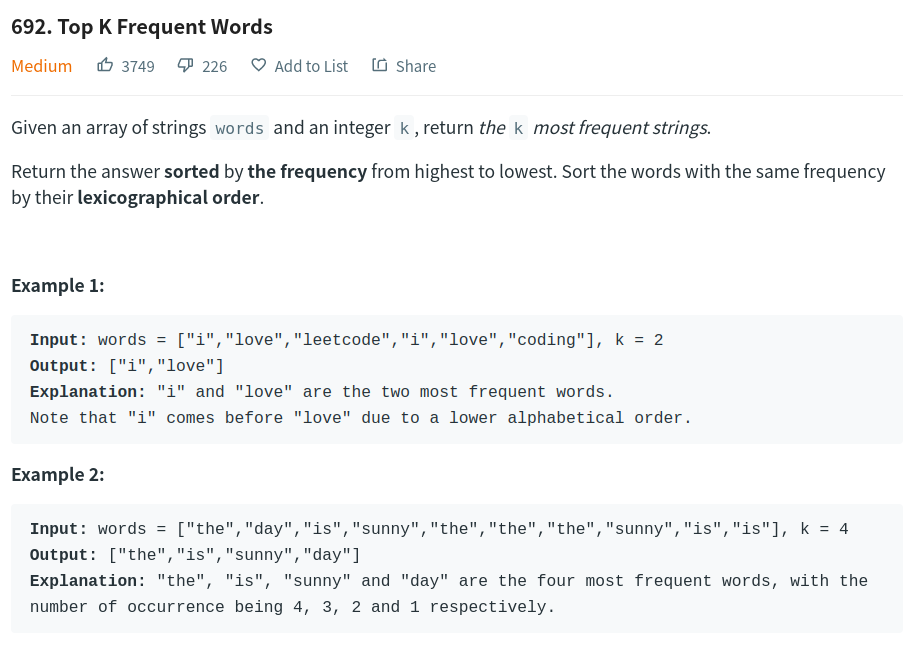
\includegraphics[width=\textwidth]{cp6/online-judge.png}
    \caption{Tasks as presented through our online tool. \red{placeholder image for now}}
    \label{fig:online-judge}
\end{figure}





\subsubsection{Procedures}
\label{cp6:evaluation-procedures}


Each experimental session lasted no more than one and a half hour; this length of time was selected based on \red{\#} pilot sessions. 
Each session began requesting participants to install a web browser plugin which we use to gather data. Setup was followed by a short tutorial explaining the experiment's purpose and describing how to use the plugin and our online judge system. We use a list sorting task that was separated from the experimental tasks and that we exclude from our analysis as the practicing example. 


We randomly assigned two tasks to a participant, presenting them in random order.  We made sure that every task was first seen by an equal number of participants. Participants were allowed to work on each task for a maximum of \red{50} minutes, and we used the remaining time to gather consent and demographics, explain experimental procedures, install a web browser plugin, and for the practice example. 



For each task, including the example, participants were asked to inspect a set of artifacts with documentation related to that task and then write a solution for the task, submitting it through our online judge system. We instructed participants that their solution did not need to pass all test cases, and we also encouraged them to compile and submit their solution at multiple points in time. Once a participant indicated that their submission was final, the system asked them to revisit the artifacts they perused and use the browser plugin to manually highlight text that assisted task completion.


We treat the first task performed by each participant as our control task.
Participants had no tool support for this task and they had to find information relevant to the task on their own. For example, using the web browser `find in page' feature.
For the second task, a tool that embedded our semantic-based technique helped participants 
highlighting text that could assist a participant in completing a task.
For this task, experimental procedures had one extra step asking a participant to rate using a Likert scale how helpful were the highlights automatically identified. This step applied to 
the highlights of one of the artifacts of a task, was determined at random. 







\subsubsection{Design}


The experiment follows a within-subjects design where the presence or absence of tool support is the experiment's \textit{independent variable}.
Dependent variables encompass:


\textit{Correctness:}  indicates whether a participant's solution fulfills the basic functionalities expected for a task. For each task, we define a subset of the test cases that a solution must pass to be considered correct. We expect that participants assisted by our tool reach a correct solution with fewer submissions. 


\textit{Completeness:} indicates the number of test cases that a participant's solution passes. 
A complete solution should pass the entire test suite for a task. Analogous to correctness, we expect that a participant assisted by our tool reaches a complete solution with fewer submissions.


\textit{Text highlighted:} represents the text that participants deemed relevant to a particular task. We use the text highlighted by participants to measure agreement on what information participants deem relevant to a task.



\textit{Perceived usefulness:} represents the extent to which a participant found the text automatically identified by a tool useful to the task at hand. We measure usefulness using a \red{three} points Likert scale similar to~\cite{nadi2020}, where a participant could select between the options:


\begin{enumerate}[label=\textit{\alph*.}]
\item the sentence is meaningful
and provides important/useful information needed to
correctly accomplish the task in question,
\item the
sentence is meaningful, but does not provide any important/useful information to correctly accomplish the task in question,
\item the sentence does not make sense to me.
\end{enumerate}




\subsubsection{Analysis}


We use each task as our unit of analysis. For each tasks, we report dependent variables within groups (i.e., control and tool-assisted) and between groups (i.e., control \textit{vs} tool-assisted)



\clearpage



\smallskip
\paragraph{\textbf{Problems with Android/Java tasks:}}

\begin{itemize}
    \item Installing and running the Android SDK is not trivial
    \item The Android emulators consume too much memory and it may be difficult to perform the tasks in certain environments
    \item Most of the tasks are visual and they don't have easy test cases that I can use to provide feedback to the students
\end{itemize}



% \subsubsection{Tasks}

% We use bugs or feature requests obtained from three popular \red{Android} GitHub repos (i.e., \textit{Omni-Notes}, \textit{K-9}, and \textit{AntennaPod}) as the tasks of our experiment. 
% We manually inspected each of the pull requests merged to the master branch in these repos and selected issues that had changes in a single file and that are related to different components core to the Android API.
% This manual inspection lead us to select the following tasks:
% \footnote{
% \textcolor{steelblue}{{\textit{AM:} one challenge with Android tasks is that, while more representative, they are harder to debug and test in a self-contained environment.
% A potential alternative are Python tasks that require using well-known modules. https://www.practicepython.org/ has examples for \texttt{beautifulsoup}}}}.

% % ---\textit{Omni-Notes}, \textit{K-9}, and \textit{AntennaPod}---



% \begin{itemize}
%     \item \texttt{Notifications}: notify users about new emails in their inbox;
%     \item \texttt{Permissions}: request user permissions to and external storage; and
%     \item \texttt{Storage}: show size of all the data used by the application.
% \end{itemize}


% While these tasks are small enough so that a student can come up with a solution in a single programming session,
% they require understanding interactions between different API components 
% and likely require the students to seek information in the Android API documentation or in community forums. 
% Therefore, we deem the tasks as appropriate to a scenario where our tool could assist a student trying to find information relevant to these tasks in a set of natural language artifacts. 


% \subsubsection{Android Application}


% Ideally, all tasks could have been selected from the same open-source project. However, our requirements on the number of classes or methods in a task's solution as well as the need that the tasks relate to core Android API components made it difficult 
% to identify a single project with such self-contained tasks. Since asking a student to familiarize themselves with running, debugging and modifying three different and complex Android applications 
% poses challenge to experimental procedures, we decided to use the 2019 Google I/O Android demo application as the core project in which the selected tasks must be implemented. 
% % \footnote{\url{https://github.com/marquesarthur/iosched}}


% The I/O Android app displays a list of conference events---sessions, office hours, app reviews, codelabs, etc.---and it lets a user filter these events by event types and by topics.
% This project has \red{[statistics about number of classes, lines, etc.]} and we believe that we can transpose the tasks that we have selected to this Android app without loss of context or complexity. 
% That is, to perform each of the selected tasks, a developer still has to make changes to a single file and they still need to consult supporting material to identify information that guides them towards 
% a solution.


